\documentclass[11pt,a4paper]{article}

\usepackage[provide=*,czech]{babel}
\usepackage[utf8]{inputenc}
\usepackage[T1]{fontenc}
\usepackage{lmodern}
\usepackage[a4paper,margin=2.5cm]{geometry}
\usepackage{booktabs}
\usepackage{tabularx}
\usepackage{longtable}
\usepackage{graphicx}
\usepackage[table]{xcolor}
\usepackage{array}
\usepackage{tikz}
\usetikzlibrary{automata,positioning,arrows.meta,shapes}
\usepackage[hidelinks]{hyperref}
\usepackage{parskip}
\usepackage{lscape}

\setlength{\emergencystretch}{3em}

\DeclareUrlCommand\id{\urlstyle{tt}}
\renewcommand{\UrlBreaks}{\do\_\do\.\do\/}

\begin{document}
\begin{titlepage}
  \centering
  {\Large Vysoké učení technické v Brně\\ Fakulta informačních technologií\par}
  \vspace{4cm}
  {\Huge Implementace překladače\\[0.3em] imperativního jazyka IFJ26\par}
  \vspace{1cm}
  {\Large Tým xpospij01, varianta vv-BVS\par}
  \vspace{2cm}

  \begin{tabular}{@{}llll@{}}
    \toprule
    Jméno a příjmení & Login & Osobní číslo & Body \\
    \midrule
    \textbf{Jan Pospíšil} & \texttt{xpospij01} & 270159 & 23\,\% \\
    Tomáš Schablický          & \texttt{xschabt00} & 281817 & 24\,\% \\
    Azíz Hammadi              & \texttt{xhammaa00} & 282529 & 21\,\% \\
    Martin Šplíchal            & \texttt{xsplicm00} & 270334 & 32\,\% \\
    \bottomrule
  \end{tabular}

  \vspace{1.5cm}
  Rozšíření: FUNEXP, BOOLTHEN, VALMEM, CONTROL\\[0.5em]
  Repozitář: \url{https://github.com/SplichalM/IFJ2026}

  \vfill
  {\large \today\par}
\end{titlepage}

\tableofcontents
\newpage

\section{Rozdělení práce}

\textbf{Tomáš Schablický}

\begin{itemize}
  \item \id{symtable.h/.c}
  \begin{itemize}
    \item datová struktura tabulky symbolů
    \item vkládání s rotacemi
  \end{itemize}

  \item \id{semantic.h/.c}
  \begin{itemize}
    \item zásobník rozsahů platnosti: \id{scope_push}, \id{scope_pop}, \id{scope_lookup}, \id{scope_declare}
    \item unikátní jména proměnných (\id{sem_unique_name}, \id{sem_copy_name}) a jejich zápis do AST
    \item vstupní bod a řízení analýzy: \id{sem_analyze}, \id{sem_check_main}, \id{sem_analyze_function}
    \item příkazy: \id{sem_block}, \id{sem_statement}, \id{sem_var_decl}, \id{sem_assign}, \id{sem_if}, \id{sem_while}, \id{sem_identifier}
    \item volání funkcí: \id{sem_call} (počet a typy argumentů, konverze argumentů)
    \item registrace vestavěných funkcí: \id{sem_add_builtin}, \id{sem_register_builtins}
    \item rozšíření:
    \begin{itemize}
      \item BOOLTHEN: \id{&&}, \id{||}, \id{!}, \id{readBoolean}, \id{Boolean} mimo podmínky
      \item VALMEM: \id{sem_member}
      \item CONTROL: \id{sem_if_expr}, převod koncového \id{if} na výraz, \id{sem_for}
    \end{itemize}
  \end{itemize}

  \item \id{codegen.h/.c}
  \begin{itemize}
    \item kostra programu: \id{gen_program}, \id{gen_function}, volací konvence přes datový zásobník
    \item deklarace lokálních proměnných: \id{gen_collect_locals}, \id{gen_pop_params}
    \item příkazy: \id{gen_block}, \id{gen_statement}, \id{gen_var_decl}, \id{gen_assign}, \id{gen_if}, \id{gen_while}, \id{gen_return}, \id{gen_body}
    \item rozšíření:
    \begin{itemize}
      \item CONTROL: \id{gen_for}, \id{gen_if_expr}, \id{gen_value_block}, \id{gen_collect_expr_locals}
    \end{itemize}
  \end{itemize}
\end{itemize}

\textbf{Azíz Hammadi}

\begin{itemize}
  \item \id{symtable.h/.c}
  \begin{itemize}
    \item inicializace, vyhledávání a uvolňování tabulky symbolů: \id{symtable_init}, \id{symtable_search}, \id{symtable_dispose}
  \end{itemize}

  \item \id{semantic.h/.c}
  \begin{itemize}
    \item typová kontrola výrazů a operátorů: \id{sem_expr_type}, \id{sem_binary_op}, \id{sem_unary_op}
    \item kompatibilita typů, přiřazení a implicitní konverze \id{Int} na \id{Double}: \id{sem_types_compatible}, \id{sem_check_assignable}, \id{sem_insert_conversion}, \id{convert_block_tail_to_double}
    \item kontrola podmínek, návratových hodnot a odvozování typů funkcí: \id{sem_check_condition}, \id{sem_return}, \id{sem_block_result}, \id{sem_check_function_result}, \id{sem_ensure_function_analyzed}
  \end{itemize}

  \item \id{codegen_expr.h/.c}
  \begin{itemize}
    \item zásobníkové generování výrazů a operátorů (\id{gen_expr}), formátování řetězcových literálů (\id{gen_push_string})
    \item volání funkcí, vestavěné funkce (\id{toInt}, \id{strLength}, \id{chr}, \id{ord}, \id{readBoolean}) a pomocná funkce \id{$builtin$subStr} (\id{gen_builtin_helpers})
    \item rozšíření:
    \begin{itemize}
    \item FUNEXP: podpora vnořeného volání funkcí ve výrazech a výrazů jako argumentů díky zásobníkové konvenci \id{gen_expr}
      \item BOOLTHEN: literály \id{Boolean}, negace \id{!}, zkratové vyhodnocování \id{&&} a \id{||}
      \item VALMEM: generování přístupu ke členům (\id{.toInt}, \id{.length}, \id{.floor}, \id{.toString})
      \item CONTROL: napojení výrazového \id{if} na \id{gen_if_expr}
    \end{itemize}
  \end{itemize}
\end{itemize}

\textbf{Jan Pospíšil}

\begin{itemize}
  \item \id{main.c}: řízení překladu (registrace vestavěných funkcí, parser, sémantika, generátor)
  \item \id{parser.h/.c}: syntaktická analýza rekurzivním sestupem, napojení callbacku \id{register_user_function}
  \item \id{precedence.h/.c}: precedenční analýza výrazů, precedenční tabulka, redukce
  \item \id{stack.h/.c}: dynamický zásobník pro precedenční analýzu
  \item \id{ast.h/.c}: uzly AST, jejich vytváření, spojování do seznamu a uvolňování
  \item rozšíření: syntaxe \id{for}, \id{if} výrazů, \id{Boolean} operátorů a přístupu ke členům
  \item \id{Makefile}, soubory \id{rozdeleni} a \id{rozsireni}
  \item code review a testování (vlastní testy, Valgrind)
  \item dokumentace: syntaktická analýza, LL gramatika, LL tabulka, precedenční tabulka
\end{itemize}

\textbf{Martin Šplíchal}

\begin{itemize}
  \item \id{lexer.h}, \id{src/lexer/lexer.c}: lexikální analýza jako konečný automat
  \begin{itemize}
    \item identifikátory a klíčová slova, číselné a řetězcové literály včetně víceřádkových
    \item vnořené komentáře, počet mezer odsazení v tokenu konce řádku
    \item rozšíření: \id{Boolean}, \id{true}, \id{false}, logické operátory, \id{for}, \id{<-}
  \end{itemize}
  \item \id{builtins_p.h/.c}: generování vestavěných funkcí \id{readLine}, \id{readInt}, \id{readDouble}, \id{print} a \id{toStr}
  \item dokumentace
\end{itemize}

\newpage

Rozdělení jsme upravili z důvodu velké pomoci Martina Šplíchala ostatním členům
týmu. To zahrnuje pomoc s prací s gitem, výpomoc na psaní vestavěných funkcí
na generátoru a psaní dokumentace. Také pomáhal při řešení různých problémů. Spravoval také GitHub a na začátku projektu rozdělil práci. Proto jsme se rozhodli Martinovi Šplíchalovi
udělit více procent (32\,\%) a ubrat tolik, kolik práce vzal od člena na sebe
a jak moc mu pomáhal (viz titulní strana).

\section{Spolupráce, testování a styl kódu}

Komunikace v týmu probíhala primárně přes chat a pravidelné hovory na Discordu.
Práce byla rozdělena rovnoměrně hned na začátku řešení projektu. Každému byla
přidělena jedna hlavní část, s tím že sémantika a generátor byly rozděleny na půl
mezi Tomáše Schablického a Azíze Hammadiho. V průběhu řešení projektu se části
práce přerozdělovaly k dalším členům týmu pro snížení zátěže na jednotlivce
a efektivnější práci.

Kód byl kontrolován Janem Pospíšilem, který následně dával zpětnou vazbu zbytku
týmu.

Testování se ujal Jan Pospíšil.

Styl jsme si předem nedomluvili, ale jednotné je pojmenování podle \id{snake_case},
funkce mají prefix svého modulu a identifikátory jsou psány anglicky.

\section{Architektura překladače}

\begin{description}
  \item[Vstup a výstup:] Překladač čte zdrojový kód ze standardního vstupu
    a na standardní výstup vypisuje kód v jazyce IFJcode26. Při úspěšném
    překladu skončí s návratovým kódem 0. Při chybě se překlad hned ukončí
    s příslušným chybovým kódem a cílový kód se nevypíše.
  \item[Řízení:] Modul \id{main.c} postupně volá parser, sémantickou analýzu
    a generátor kódu. Zároveň drží tabulku funkcí, do které před parsováním
    vloží vestavěné funkce, a předává ji parseru a sémantické analýze.
  \item[Lexikální a syntaktická analýza:] Parser si od lexeru bere tokeny
    na vyžádání. Uzly AST pro definice funkcí a příkazy tvoří sám. Na místě
    výrazu volá precedenční analýzu, která sestaví podstrom výrazu. Volání
    funkcí a if-výrazy uvnitř výrazu přitom zpětně zpracuje parser.
  \item[Callback:] Po načtení každé definice funkce parser zavolá callback
    \id{register_user_function} ze sémantického modulu. Ten funkci i s typy
    parametrů a návratovým typem vloží do tabulky funkcí. Sémantická analýza
    proto při svém spuštění zná všechny funkce a funguje i volání funkce
    definované později.
  \item[Sémantická analýza:] Prochází a kontroluje AST. Pro funkce používá
    tabulku funkcí, pro proměnné zásobník tabulek symbolů podle rozsahů
    platnosti. Zároveň doplní do AST datové typy, unikátní jména proměnných,
    implicitní konverze a odvozené návratové typy funkcí bez explicitního
    typu. Výsledkem je dekorovaný AST.
  \item[Generátor:] Z dekorovaného AST vypisuje výsledný kód. Funkce a příkazy
    generuje \id{codegen.c}, výrazy \id{codegen_expr.c}. Vestavěné funkce
    \id{readLine}, \id{readInt}, \id{readDouble}, \id{print} a \id{toStr}
    generuje \id{builtins_p.c}, ostatní vestavěné funkce \id{codegen_expr.c}.
\end{description}

\begin{figure}[p]
  \centering
  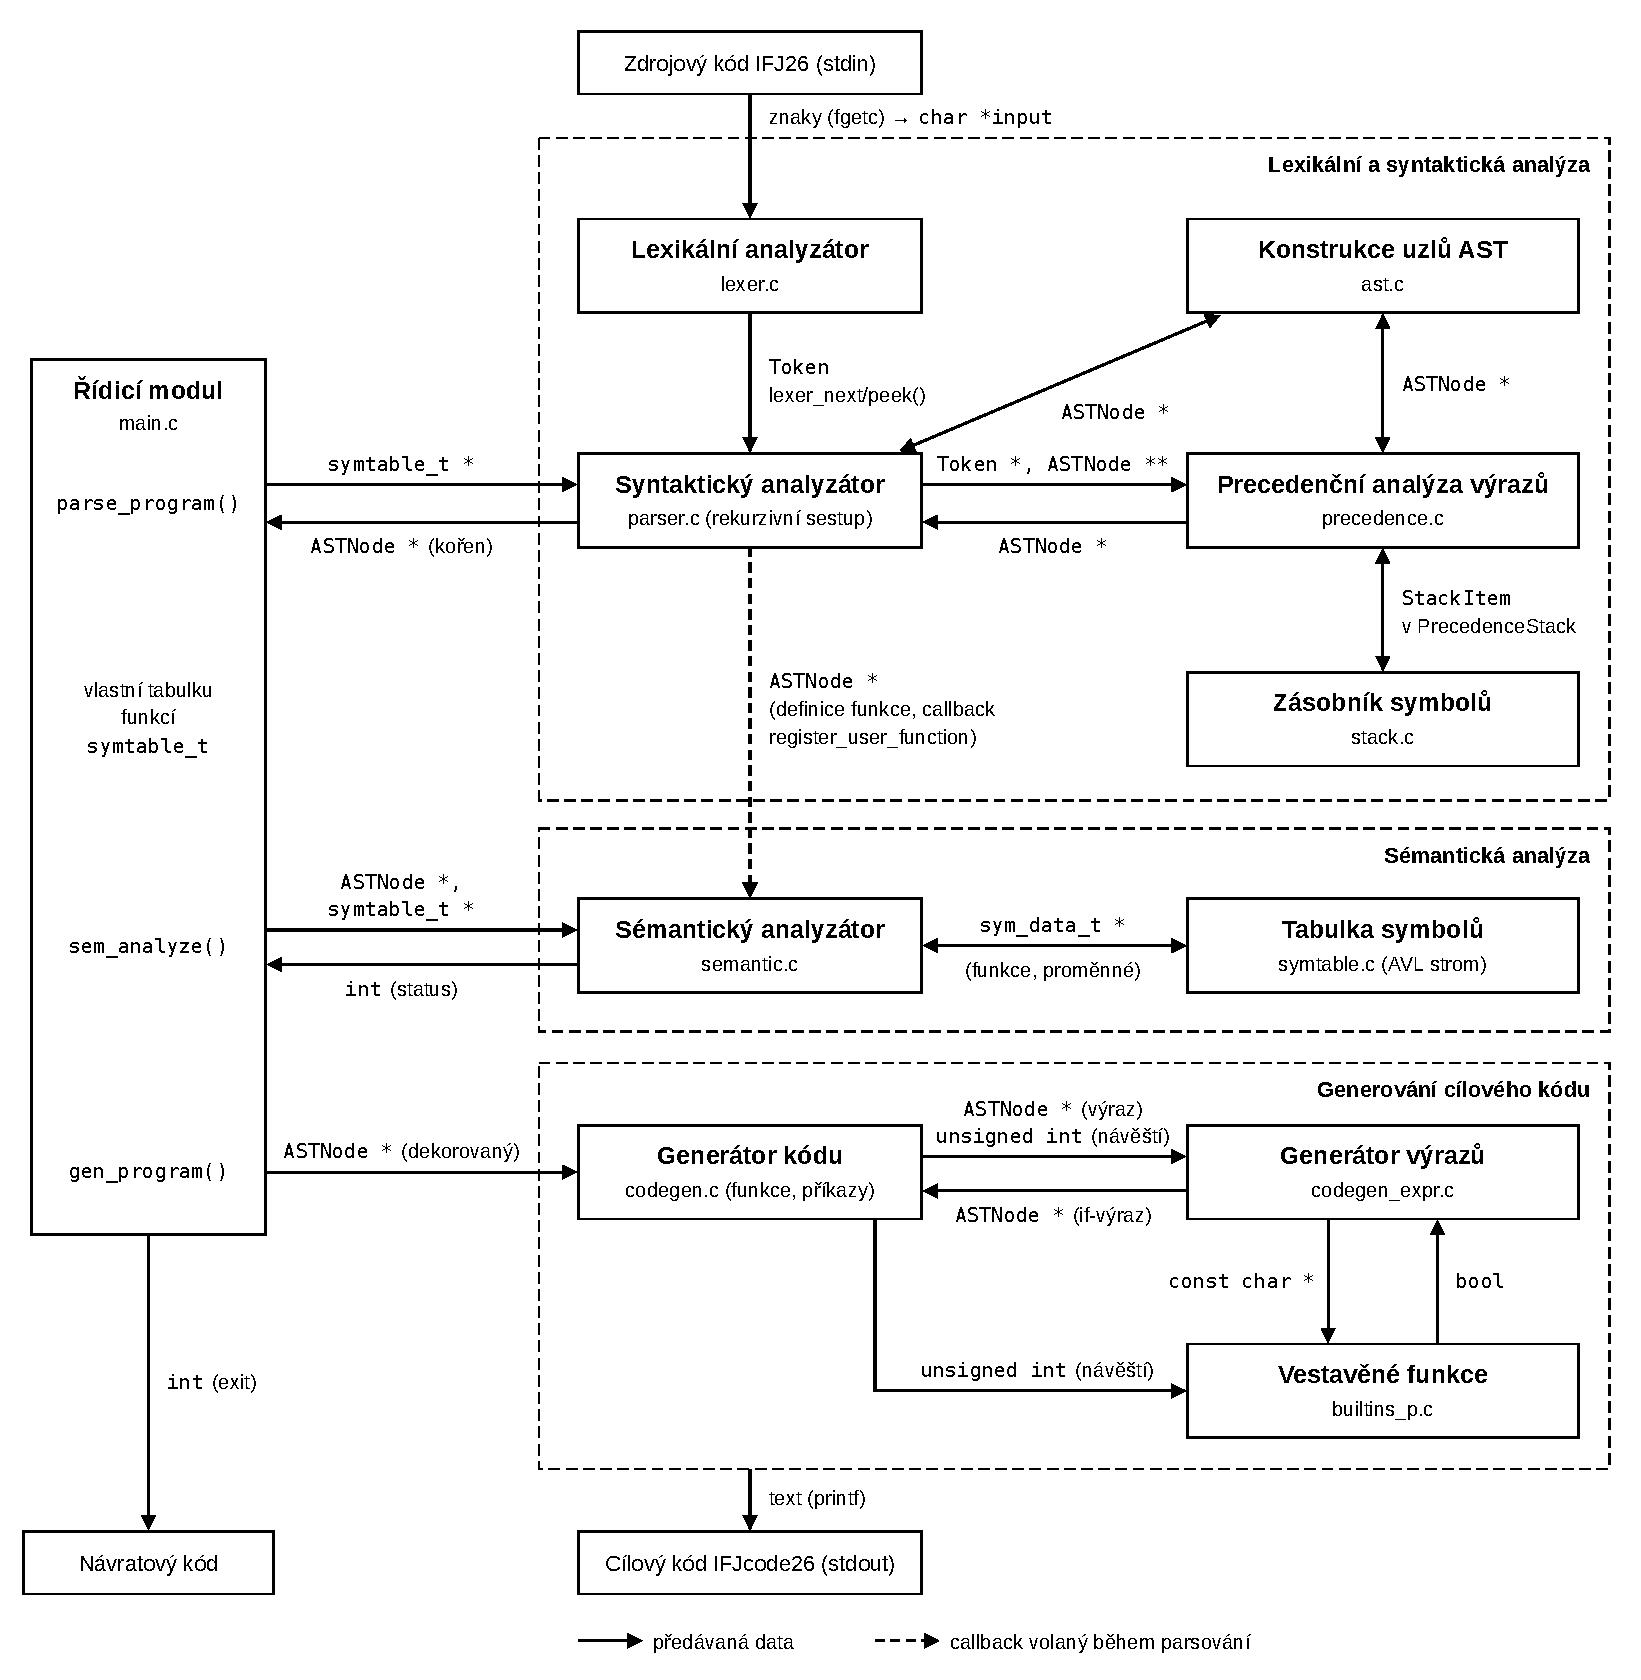
\includegraphics[width=\textwidth,height=0.8\textheight,keepaspectratio]{blokove_schema.pdf}
  \caption{Architektura překladače}
  \label{fig:architektura}
\end{figure}

\newpage

\section{Lexikální analýza}

Lexer v souboru \texttt{src/lexer/lexer.c} čte zdrojový program ze standardního
vstupu a předává parseru tokeny. Rozhraní je v \texttt{include/lexer.h}.

\paragraph{Čtení tokenů.}
\texttt{lexer\_init()} načte celý vstup do paměti a \texttt{lexer\_free()}
ho uvolní. \texttt{lexer\_next()} přečte další token. Funkce
\texttt{lexer\_peek()} ho vrátí bez posunu ve vstupu. Parser uvolní text
z pole \texttt{context}, až ho nepotřebuje.

\paragraph{Znaky a řádky.}
Lexer načte celé jméno a pak ho porovná se seznamem klíčových slov.
U vnořených komentářů počítá jejich začátky a konce. S tokenem konce
řádku předá počet mezer na začátku dalšího řádku. Parser podle něj
kontroluje odsazení bloků.

\paragraph{Chyby.}
Lexer vrátí \texttt{TOKEN\_ERROR} s kódem~1 pro chybný zápis a~99 pro
vnitřní chybu, třeba při nedostatku paměti. Kód~2 vrátí, pokud za koncem
víceřádkového komentáře najde na stejném řádku znak, který tam být nemá.

\paragraph{Rozšíření.}
Pro \texttt{BOOLTHEN} lexer rozpoznává \texttt{Boolean}, \texttt{true},
\texttt{false} a logické operátory. Pro \texttt{CONTROL} přidává
\texttt{for} a \texttt{<-}. \texttt{FUNEXP} a \texttt{VALMEM}
používají stejné tokeny jako základ.

\newgeometry{margin=9mm}
\begin{landscape}
  \thispagestyle{empty}
\begingroup

\newcommand{\znak}[1]{\texttt{#1}}
\newcommand{\token}[1]{\texttt{\detokenize{#1}}}
\newcommand{\nazev}[1]{%
  \node[anchor=north west, font=\sffamily\bfseries\fontsize{10}{11}\selectfont]
    at (3,2.2) {#1};
}

\tikzset{
  ramecek/.style={draw=black!60, line width=.45pt},
  stav/.style={circle, draw, minimum size=7.7mm, inner sep=0pt},
  prijeti/.style={stav, double, double distance=.75pt},
  sipka/.style={-{Stealth[length=1.8mm, width=1.3mm]}, line width=.45pt},
  popis/.style={font=\sffamily\fontsize{7.5}{9}\selectfont, inner sep=1pt, align=center},
  vysvetlivka/.style={anchor=north west, align=left, inner sep=0pt,
    font=\sffamily\fontsize{7.5}{9.25}\selectfont}
}

\vspace*{-\topskip}
\noindent\begin{tikzpicture}[x=1mm, y=-1mm, font=\sffamily\fontsize{8.5}{10}\selectfont]

\draw[ramecek] (0,0) rectangle (274.5,53);
\draw[ramecek] (105.5,0) -- (105.5,53);
\draw[ramecek] (0,53) -- (0,131) -- (274.5,131) -- (274.5,53);
\draw[ramecek] (181,53) -- (181,131);
\draw[ramecek] (0,131) -- (0,182) -- (274.5,182) -- (274.5,131);
\draw[ramecek] (181,131) -- (181,182);

\nazev{Identifikátory a klíčová slova}

\node[stav] (jmeno) at (83,26) {$s_{\rm jm}$};
\node[stav] (druhJmena) at (54,26) {$s_{\rm typ}$};
\node[prijeti] (pravdivostni) at (17,14) {$s_{\rm bool}$};
\node[prijeti] (klicove) at (17,26) {$s_{\rm kw}$};
\node[prijeti] (identifikator) at (17,38.5) {$s_{\rm id}$};
\node[stav] (chybaJmena) at (54,41) {$s_{\rm err1}$};

\draw[sipka] (jmeno.133) to[out=133,in=47,looseness=4.4]
  node[popis,above] {$P$, $C$, \token{_}} (jmeno.47);
\draw[sipka] (jmeno) -- node[popis,above] {mimo $P$, $C$, \token{_}\\nebo EOF} (druhJmena);
\draw[sipka] (druhJmena) -- (pravdivostni);
\node[popis] at (35,16.6) {\znak{true}, \znak{false}};
\draw[sipka] (druhJmena) -- node[popis,above] {klíčové slovo} (klicove);
\draw[sipka] (druhJmena) -- (identifikator);
\node[popis] at (35,36.8) {jiné jméno};
\draw[sipka] (druhJmena) -- node[popis,right,xshift=1mm] {jen \token{_}} (chybaJmena);

\node[vysvetlivka] at (60,3.2) {$P$ = A--Z, a--z\quad $C$ = 0--9};
\node[vysvetlivka] at (75,45) {$s_{\rm jm}$ = čtení jména\\$s_{\rm typ}$ = určení typu};
\node[vysvetlivka] at (3,46) {%
  $s_{\rm id}$ = \token{TOKEN_IDENTIFIER}, $s_{\rm kw}$ = \token{TOKEN_KEYWORD}\\
  $s_{\rm bool}$ = \token{TOKEN_BOOL}};

\begin{scope}[xshift=105.5mm]
\nazev{Začátek čtení, lomítko a komentáře}

\node[stav] (zacatek) at (13,22) {$s_0$};
\node[prijeti] (deleni) at (35,22) {$s_{\rm div}$};
\node[stav] (neznamyZnak) at (45,12.6) {$s_{\rm err1}$};
\node[stav] (radkovy) at (71,17) {$s_{\rm rad}$};
\node[stav] (blok) at (65,34) {$s_{\rm blok}$};
\node[stav] (zaBlokem) at (107,34) {$s_{\rm za}$};
\node[prijeti] (eol) at (150,17) {$s_{\rm eol}$};
\node[stav] (chybaKomentare) at (87,46) {$s_{\rm err1}$};
\node[stav] (chybaDva) at (150,34) {$s_{\rm err2}$};

\draw[sipka] (4,22) -- (zacatek);
\draw[sipka] (zacatek.133) to[out=133,in=47,looseness=4.4]
  node[popis,above] {$W$} (zacatek.47);
\draw[sipka] (zacatek) -- (neznamyZnak);
\node[popis] at (29,12) {neznámý znak};
\draw[sipka] (zacatek) -- node[popis,above] {\znak{/}} (deleni);
\draw[sipka] (deleni) -- node[popis,above] {\znak{/}} (radkovy);
\draw[sipka] (deleni) -- node[popis,above] {\znak{*}} (blok);
\node[popis] at (47,31.5) {$d\gets1$, $L\gets0$};

\draw[sipka] (radkovy.133) to[out=133,in=47,looseness=4.4]
  node[popis,above] {kromě LF} (radkovy.47);
\draw[sipka] (radkovy) -- node[popis,below] {LF, EOF} (eol);

\draw[sipka] (blok.133) to[out=133,in=47,looseness=4.4]
  node[popis,above] {tělo komentáře} (blok.47);
\draw[sipka] (blok) -- node[popis,above] {\znak{*/}, $d=1$, $L=1$} (zaBlokem);
\draw[sipka, rounded corners=1.7mm] (blok.south) -- (65,45) --
  node[popis,above,pos=.33] {\znak{*/}, $d=1$, $L=0$} (13,45) -- (zacatek.south);
\draw[sipka] (blok) -- (chybaKomentare);
\node[popis] at (81,39) {EOF};

\draw[sipka] (zaBlokem.133) to[out=133,in=47,looseness=4.4]
  node[popis,above] {mezera, tabulátor, CR} (zaBlokem.47);
\draw[sipka] (zaBlokem) -- (eol);
\node[popis] at (130,29.5) {LF, EOF};
\draw[sipka] (zaBlokem) -- node[popis,below] {jiný znak} (chybaDva);

\node[vysvetlivka] at (93,2.8) {%
  LF = nový řádek, EOF = konec vstupu, CR = \znak{\textbackslash r}\\
  $d$ = hloubka vnoření, $L$ = výskyt LF uvnitř komentáře\\
  \znak{/*} zvýší $d$, vnitřní \znak{*/} sníží $d$, LF nastaví $L=1$};
\node[vysvetlivka] at (104,39) {%
  $s_{\rm rad}$ = řádkový, $s_{\rm blok}$ = blokový komentář\\
  $s_{\rm za}$ = kontrola za blokovým komentářem\\
  $s_{\rm div}$ = operátor \znak{/}, $s_{\rm eol}$ = \token{TOKEN_EOL}};
\end{scope}

\draw[sipka] (zacatek.225) .. controls (109,34) and (96,32) .. (jmeno.east);
\node[popis] at (97.5,34) {$P$ nebo \token{_}};

\begin{scope}[shift={(0,53)}]
\nazev{Celá a desetinná čísla}

\node[stav] (celaCast) at (84,27) {$s_{\rm cel}$};
\node[stav] (desetinnaCast) at (153,28) {$s_{\rm des}$};
\node[stav] (exponent) at (117,48) {$s_{\rm exp}$};
\node[stav] (kontrolaDouble) at (90,62) {$s_{\rm kd}$};
\node[prijeti] (celeCislo) at (22,27) {$s_{\rm int}$};
\node[prijeti] (desetinneCislo) at (42,62) {$s_{\rm dbl}$};
\node[stav] (chybaInt) at (70,41) {$s_{\rm err1}$};
\node[stav] (chybaDouble) at (65,55) {$s_{\rm err1}$};

\draw[sipka] (celaCast.133) to[out=133,in=47,looseness=4.4]
  node[popis,above] {$C$, \token{_}} (celaCast.47);
\draw[sipka] (desetinnaCast.55) to[out=55,in=305,looseness=4.4]
  node[popis,right] {$C$, \token{_}} (desetinnaCast.305);
\draw[sipka] (exponent.310) to[out=310,in=230,looseness=4.4]
  node[popis,below] {$C$, \token{_}} (exponent.230);

\draw[sipka] (celaCast) -- node[popis,above] {$T$} (desetinnaCast);
\draw[sipka] (celaCast) -- (exponent);
\node[popis] at (100,32) {\znak{e/E} $[\pm]$};
\draw[sipka] (desetinnaCast) -- (exponent);
\node[popis] at (137.5,32) {\znak{e/E} $[\pm]$};

\draw[sipka] (celaCast) -- node[popis,above] {konec Int, platný zápis} (celeCislo);
\draw[sipka] (celaCast) -- (chybaInt);
\node[popis, anchor=west] at (78,39) {konec Int,\\vadný zápis};

\draw[sipka] (exponent) -- (kontrolaDouble);
\node[popis] at (94,51) {mimo $C$, \token{_}\\nebo EOF};
\draw[sipka, rounded corners=1.5mm] (desetinnaCast.south) -- (153,62) --
  node[popis,below] {mimo $C$, \token{_}, \znak{e/E} nebo EOF} (kontrolaDouble.east);
\draw[sipka] (kontrolaDouble) -- node[popis,above] {platné, volitelné \znak{d/D}} (desetinneCislo);
\draw[sipka] (kontrolaDouble) -- (chybaDouble);
\node[popis] at (78,55) {vadný Double};

\node[vysvetlivka] at (9,9) {%
  $C$ = 0--9, $P$ = A--Z, a--z, $[\pm]$ = volitelné znaménko\\
  $T$ = tečka před EOF nebo před znakem mimo $P$, \token{_}\\
  Konec Int = EOF nebo vstup mimo $C$, \token{_}, \znak{e/E} a $T$};
\node[vysvetlivka] at (9,33.5) {%
  Platný Int má \token{_} jen mezi číslicemi,\\
  úvodní nulu jen u nulové hodnoty\\
  a vejde se do 64bitového celého čísla.};
\node[vysvetlivka] at (9,47) {%
  $s_{\rm cel}$ = celá část, $s_{\rm des}$ = desetinná část\\
  $s_{\rm exp}$ = exponent, $s_{\rm kd}$ = kontrola Double};
\node[vysvetlivka] at (9,72) {$s_{\rm int}$ = \token{TOKEN_INT}, $s_{\rm dbl}$ = \token{TOKEN_DOUBLE}};
\node[vysvetlivka] at (97,70) {%
  Po tečce a v exponentu musí být číslice. \token{_} jen mezi číslicemi.\\
  Chyba = \znak{f/F} bez dalšího $P$, $C$, \token{_}, přetečení nebo podtečení na nulu.};
\end{scope}

\draw[sipka] (zacatek.244) .. controls (107,40) and (105,68) .. (celaCast.18);
\node[popis] at (99,73) {$C$};
\draw[sipka, rounded corners=1.7mm] (zacatek.259) .. controls (116,36) and (116,47) ..
  (121,60) -- node[popis,below] {\znak{.}, následuje $C$} (153,60) -- (desetinnaCast.north);

\begin{scope}[shift={(181,53)}]
\nazev{Řetězcové literály}

\node[stav] (uvozovka) at (77,13.5) {$s_{\rm uv}$};
\node[stav] (jednoradkovy) at (40,27) {$s_{\rm jr}$};
\node[stav] (escape) at (13,37) {$s_{\rm esc}$};
\node[stav] (viceradkovy) at (75,37) {$s_{\rm vr}$};
\node[prijeti] (retezec) at (49,55) {$s_{\rm str}$};
\node[stav] (chybaRetezce) at (23,55) {$s_{\rm err1}$};
\node[stav] (chybaViceradkoveho) at (75,56) {$s_{\rm err1}$};

\draw[sipka] (uvozovka) -- (jednoradkovy);
\node[popis] at (57,13.5) {bez dalších dvou \znak{"}};
\draw[sipka] (uvozovka) -- node[popis,right] {\znak{""}} (viceradkovy);
\draw[sipka] (jednoradkovy.133) to[out=133,in=47,looseness=4.4]
  node[popis,above] {$B$} (jednoradkovy.47);
\draw[sipka] (jednoradkovy.173) -- node[popis,above] {\znak{\textbackslash}} (escape.70);
\draw[sipka] (escape.355) -- node[popis,below] {$E$} (jednoradkovy.224);
\draw[sipka] (jednoradkovy) -- node[popis,right] {\znak{"}} (retezec);
\draw[sipka] (jednoradkovy) -- (chybaRetezce);
\node[popis,anchor=west] at (31.4,46.5) {LF, NUL,\\EOF};
\draw[sipka] (escape) -- (chybaRetezce);
\node[popis,anchor=west] at (3,47.6) {mimo $E$\\nebo EOF};

\draw[sipka] (viceradkovy.55) to[out=55,in=305,looseness=4.1]
  node[popis,right] {obsah\\doslova} (viceradkovy.305);
\draw[sipka] (viceradkovy) -- (retezec);
\node[popis] at (59,40.1) {\znak{"""} a další \znak{"}};
\draw[sipka] (viceradkovy) -- node[popis,right] {NUL, EOF} (chybaViceradkoveho);

\node[vysvetlivka] at (3,62) {%
  $B$ = znak mimo \znak{"}, \znak{\textbackslash}, LF a NUL. NUL = \znak{\textbackslash 0}.\\
  $E$ = \znak{\textbackslash}, \znak{"}, \znak{n}, \znak{r}, \znak{t}. $s_{\rm esc}$ = zpracování escape sekvence.\\
  $s_{\rm uv}$ = po první \znak{"}. $s_{\rm jr}$ / $s_{\rm vr}$ = jednořádkový / víceřádkový.\\
  $s_{\rm str}$ = \token{TOKEN_STRING}. Z řady \znak{"} uzavírají víceřádkový zápis poslední tři.};
\end{scope}

\draw[sipka, rounded corners=1.8mm] (zacatek.291) .. controls (123,32) and (126,43) ..
  (126,51) -- (258,51) -- node[popis,right] {\znak{"}} (uvozovka.north);

\begin{scope}[shift={(0,131)}]
\nazev{Operátory, oddělovače a anotace}

\node[stav] (znacka) at (156,12) {$s_{\rm zn}$};
\node[prijeti] (kratkyOperator) at (107,14) {$s_{\rm op1}$};
\node[prijeti] (operator) at (65,12) {$s_{\rm op}$};
\node[stav] (parOperatoru) at (102,29.5) {$s_{\rm par}$};
\node[stav] (chybaOperatoru) at (129,30.5) {$s_{\rm err1}$};
\node[prijeti] (oddelovac) at (168,31) {$s_{\rm odd}$};
\node[stav] (zavinac) at (53,33) {$s_{\rm zav}$};
\node[prijeti] (anotace) at (15,24.5) {$s_{\rm an}$};
\node[stav] (chybaAnotace) at (15,39) {$s_{\rm err1}$};

\draw[sipka, rounded corners=1.5mm] (znacka.110) -- (151,4.2) --
  node[popis,above] {\znak{+ - *}} (65,4.2) -- (operator.north);
\draw[sipka] (znacka) -- node[popis,above] {\znak{= < > !}} (kratkyOperator);
\draw[sipka] (kratkyOperator) -- node[popis,above] {\znak{=} nebo \znak{-} po \znak{<}} (operator);

\draw[sipka] (znacka) -- node[popis,below] {\znak{\& |}} (parOperatoru);
\draw[sipka] (parOperatoru) -- (operator);
\node[popis] at (80,24.5) {stejný znak};
\draw[sipka] (parOperatoru) -- (chybaOperatoru);
\node[popis] at (115.5,34.5) {jiný znak, EOF};

\draw[sipka] (znacka) -- node[popis,right] {$O$} (oddelovac);
\draw[sipka, rounded corners=1.6mm] (znacka.242) -- (148,38) --
  node[popis,below] {\znak{@}} (58,38) -- (zavinac.312);
\draw[sipka] (zavinac) -- node[popis,above] {$A$} (anotace);
\draw[sipka] (zavinac) -- node[popis,below] {bez $A$} (chybaAnotace);

\node[vysvetlivka] at (3,44) {%
  $A$ = \znak{main} před EOF nebo znakem mimo $P$, $C$, \token{_}.\\
  $s_{\rm zav}$ = po \znak{@}, $s_{\rm an}$ = \token{TOKEN_ANNOTATION}};
\node[vysvetlivka] at (68,41.5) {%
  $s_{\rm zn}$ = volba značky, $s_{\rm par}$ = po \znak{\&} nebo \znak{|}\\
  $s_{\rm op1}$, $s_{\rm op}$ = \token{TOKEN_OPERATOR}\\
  $s_{\rm odd}$ = \token{TOKEN_SEPARATOR}};
\node[vysvetlivka] at (124,41) {%
  $O$ = \znak{( ) , : ;} nebo \znak{.} bez číslice za ní.\\
  $Z$ = \znak{+ - * = < > ! \& | @} nebo $O$.\\
  $P$ = A--Z, a--z, $C$ = 0--9.};
\end{scope}

\draw[sipka, rounded corners=1.8mm] (zacatek.318) .. controls (125,30) and (130,46) ..
  (132,55.5) -- (177,55.5) -- (177,137) -- node[popis,above] {$Z$} (157,137) -- (znacka.north);

\begin{scope}[shift={(181,131)}]
\nazev{Bílé znaky, odsazení a EOF}

\node[stav] (konecRadkuVstupu) at (14,16) {$s_{\rm k}$};
\node[stav] (odsazeni) at (48,24) {$s_{\rm ods}$};
\node[prijeti] (fyzickyKonecRadku) at (80,29) {$s_{\rm lf}$};
\node[prijeti] (konecVstupu) at (77,11) {$s_{\rm eof}$};
\node[stav] (chybaOdsazeni) at (15,33.5) {$s_{\rm err1}$};

\draw[sipka] (konecRadkuVstupu) -- node[popis,above] {EOF} (konecVstupu);
\draw[sipka] (konecRadkuVstupu) -- node[popis,above] {LF} (odsazeni);
\draw[sipka] (konecRadkuVstupu) -- (chybaOdsazeni);
\node[popis,anchor=west,align=left] at (19,27.5) {TAB v odsazení\\před kódem};

\draw[sipka] (odsazeni.310) to[out=310,in=230,looseness=4.3]
  node[popis,below] {jen $W$ s TAB, pak LF} (odsazeni.230);
\draw[sipka] (odsazeni) -- (fyzickyKonecRadku);
\node[popis] at (66,20.6) {obsah, EOF\\nebo LF bez TAB};

\node[vysvetlivka,font=\sffamily\fontsize{7.5}{8.4}\selectfont] at (3,38.5) {%
  $W$ = mezera, TAB (\znak{\textbackslash t}), CR. TAB v odsazení si lexer pamatuje.\\
  $K$ = LF, EOF nebo TAB v odsazení před kódem.\\
  $s_{\rm k}$ = kontrola po $W$ a komentářích, $s_{\rm ods}$ = počet mezer za LF.\\
  $s_{\rm lf}$ = \token{TOKEN_EOL} s počtem mezer, $s_{\rm eof}$ = \token{TOKEN_EOF}.};
\end{scope}

\draw[sipka, rounded corners=1.5mm] (zacatek.339) .. controls (129,31) and (133,45) ..
  (135,57.7) -- (179.1,57.7) -- (179.1,147) -- node[popis,above] {$K$} (konecRadkuVstupu.west);

\node[overlay, vysvetlivka, anchor=south west] at (0,191) {%
  $s_{\rm err1}$ = \token{TOKEN_ERROR} s kódem 1. Každé vyobrazení $s_{\rm err1}$ značí tentýž stav.\\
  $s_{\rm err2}$ = \token{TOKEN_ERROR} s kódem 2. Kód 99 značí interní chybu.};
\node[overlay, vysvetlivka, anchor=south west] at (118,191) {%
  Po přeskočení $W$ a komentářů má $K$ přednost před běžnými tokeny.\\
  LF za \znak{//} se zpracuje jako běžný LF. Na EOF za \znak{//} je odsazení 0.};

\end{tikzpicture}
\par
\endgroup
\end{landscape}
\restoregeometry

\section{Syntaktická analýza}
Syntaktický analyzátor kombinuje rekurzivní sestup (shora dolů) s precedenční analýzou. Rekurzivní sestup postupně zpracovává strukturu programu a výrazy předává zásobníkovému analyzátoru, který je řízený dvourozměrnou precedenční tabulkou. Vstupním bodem parseru je funkce \texttt{parse\_program}, která je volána z \texttt{main.c}. Na začátku inicializuje lexer a zpracuje prolog, potom postupně načítá definice funkcí, jejich parametry a těla. Vnořené bloky zpracovává vzájemným voláním funkcí pro příkazy a bloky.

Parser si uchovává aktuální token a prostřednictvím \texttt{lexer\_next} získává další token. Při rozlišování přiřazení a volání funkce využívá také funkci \texttt{lexer\_peek}, která umožňuje nahlédnout na následující token bez posunu vstupu. Hranice bloků určuje pomocí odsazení, o kterém dostává informaci v tokenech EOL.

Během syntaktické analýzy parser vytváří AST, který obsahuje definice funkcí, výrazy a příkazy. Po zpracování každé definice funkce zavolá registrační funkci sémantického analyzátoru \texttt{register\_\allowbreak user\_\allowbreak function}, která uloží informace o funkci a ukazatel na její uzel do tabulky symbolů. Díky tomu má sémantika k dispozici tabulku všech definovaných funkcí a nemusí provádět samostatný průchod pro sběr jejich definic. Může tak zpracovat i volání funkce, jejíž definice se nachází až za jejím použitím.

\subsection{Zpracování výrazů}
Výrazy jsou zpracovávány syntaktickou analýzou zdola nahoru pomocí dynamického zásobníku a dvourozměrné precedenční tabulky. Řádek tabulky vybíráme podle nejvyššího terminálu na zásobníku a sloupec podle aktuálního vstupního symbolu. Operátory, které mají stejnou prioritu, jsou dány do skupiny.

Podle relace v precedenční tabulce se provede buď posun, nebo redukce. Při relaci $<$ analyzátor vloží na zásobník značku začátku redukovaného úseku a vstupní symbol. Při relaci $=$ vloží pouze vstupní symbol. Relace $>$ vyvolá funkci \texttt{reduce}, která zpracuje úsek za poslední značkou, vytvoří odpovídající uzel AST a nahradí úsek výsledným výrazem. Vstupní token při redukci zůstává stejný.

Volání funkcí a výrazové \texttt{if} zpracovávají funkce parseru a jejich AST se dále používá jako operand. Výraz končí podle místa svého použití, například před čárkou mezi argumenty nebo před klíčovým slovem \texttt{then}. Tuto hranici v tabulce zastupuje symbol \texttt{\$}. Pokud nad počáteční značkou zásobníku zůstane jediný výsledný výraz a vstup dosáhne jeho hranice, je analýza úspěšná. Nepovolená akce v tabulce nebo úsek, který nelze zredukovat, znamená syntaktickou chybu.


\subsection{LL gramatika řídicí části}

\begingroup
\small
\setlength{\tabcolsep}{2pt}
\renewcommand{\arraystretch}{1.03}
\begin{longtable}{@{}r@{\quad}>{\raggedright\arraybackslash}p{0.91\linewidth}@{}}
\hline Č. & Pravidlo \\ \hline
\endfirsthead
\hline Č. & Pravidlo \\ \hline
\endhead
\hline\endfoot
1 & \texttt{\textless{}program\textgreater{}} $\rightarrow$ \texttt{\textless{}eol\_opt\textgreater{}} \texttt{\textless{}prolog\textgreater{}} \texttt{\textless{}eol\_plus\textgreater{}} \texttt{\textless{}functions\textgreater{}} \\
2 & \texttt{\textless{}prolog\textgreater{}} $\rightarrow$ \texttt{"import"} \texttt{"ifj26"} \texttt{"."} \texttt{"*"} \\
3 & \texttt{\textless{}eol\_opt\textgreater{}} $\rightarrow$ \texttt{EOL} \texttt{\textless{}eol\_opt\textgreater{}} \\
4 & \texttt{\textless{}eol\_opt\textgreater{}} $\rightarrow$ $\varepsilon$ \\
5 & \texttt{\textless{}eol\_plus\textgreater{}} $\rightarrow$ \texttt{EOL} \texttt{\textless{}eol\_opt\textgreater{}} \\
6 & \texttt{\textless{}functions\textgreater{}} $\rightarrow$ \texttt{\textless{}function\textgreater{}} \\
7 & \texttt{\textless{}functions\textgreater{}} $\rightarrow$ \texttt{EOF} \\
8 & \texttt{\textless{}function\textgreater{}} $\rightarrow$ \texttt{\textless{}main\_opt\textgreater{}} \texttt{"def"} \texttt{ID} \texttt{"("} \texttt{\textless{}eol\_opt\textgreater{}} \texttt{\textless{}parametrs\textgreater{}} \texttt{")"} \texttt{\textless{}return\_type\textgreater{}} \texttt{"="} \texttt{\textless{}function\_body\textgreater{}} \\
9 & \texttt{\textless{}main\_opt\textgreater{}} $\rightarrow$ \texttt{"@main"} \texttt{\textless{}eol\_opt\textgreater{}} \\
10 & \texttt{\textless{}main\_opt\textgreater{}} $\rightarrow$ $\varepsilon$ \\
11 & \texttt{\textless{}parametrs\textgreater{}} $\rightarrow$ \texttt{\textless{}parametr\textgreater{}} \texttt{\textless{}parametrs\_tail\textgreater{}} \\
12 & \texttt{\textless{}parametrs\textgreater{}} $\rightarrow$ $\varepsilon$ \\
13 & \texttt{\textless{}parametr\textgreater{}} $\rightarrow$ \texttt{ID} \texttt{\textless{}eol\_opt\textgreater{}} \texttt{":"} \texttt{\textless{}eol\_opt\textgreater{}} \texttt{\textless{}type\textgreater{}} \\
14 & \texttt{\textless{}parametrs\_tail\textgreater{}} $\rightarrow$ \texttt{EOL} \texttt{\textless{}parametrs\_tail\textgreater{}} \\
15 & \texttt{\textless{}parametrs\_tail\textgreater{}} $\rightarrow$ \texttt{","} \texttt{\textless{}parametr\_or\_end\textgreater{}} \\
16 & \texttt{\textless{}parametrs\_tail\textgreater{}} $\rightarrow$ $\varepsilon$ \\
17 & \texttt{\textless{}parametr\_or\_end\textgreater{}} $\rightarrow$ \texttt{\textless{}parametr\textgreater{}} \texttt{\textless{}parametrs\_tail\textgreater{}} \\
18 & \texttt{\textless{}parametr\_or\_end\textgreater{}} $\rightarrow$ \texttt{EOL} \texttt{\textless{}eol\_opt\textgreater{}} \texttt{\textless{}parametrs\textgreater{}} \\
19 & \texttt{\textless{}type\textgreater{}} $\rightarrow$ \texttt{"Unit"} \\
20 & \texttt{\textless{}type\textgreater{}} $\rightarrow$ \texttt{"String"} \\
21 & \texttt{\textless{}type\textgreater{}} $\rightarrow$ \texttt{"Int"} \\
22 & \texttt{\textless{}type\textgreater{}} $\rightarrow$ \texttt{"Double"} \\
23 & \texttt{\textless{}type\textgreater{}} $\rightarrow$ \texttt{"Boolean"} \\
24 & \texttt{\textless{}return\_type\textgreater{}} $\rightarrow$ \texttt{":"} \texttt{\textless{}type\textgreater{}} \\
25 & \texttt{\textless{}return\_type\textgreater{}} $\rightarrow$ $\varepsilon$ \\
26 & \texttt{\textless{}function\_body\textgreater{}} $\rightarrow$ \texttt{EXPR} \texttt{\textless{}function\_next\textgreater{}} \\
27 & \texttt{\textless{}function\_body\textgreater{}} $\rightarrow$ \texttt{\textless{}suite\textgreater{}} \texttt{\textless{}functions\textgreater{}} \\
28 & \texttt{\textless{}function\_next\textgreater{}} $\rightarrow$ \texttt{\textless{}eol\_plus\textgreater{}} \texttt{\textless{}functions\textgreater{}} \\
29 & \texttt{\textless{}function\_next\textgreater{}} $\rightarrow$ \texttt{EOF} \\
30 & \texttt{\textless{}suite\textgreater{}} $\rightarrow$ \texttt{\textless{}eol\_plus\textgreater{}} \texttt{INDENT} \texttt{\textless{}block\textgreater{}} \texttt{DEDENT} \\
31 & \texttt{\textless{}block\textgreater{}} $\rightarrow$ \texttt{\textless{}simple\_core\textgreater{}} \texttt{\textless{}block\_after\_simple\textgreater{}} \\
32 & \texttt{\textless{}block\textgreater{}} $\rightarrow$ \texttt{\textless{}if\_stmt\textgreater{}} \\
33 & \texttt{\textless{}block\textgreater{}} $\rightarrow$ \texttt{\textless{}while\_stmt\textgreater{}} \texttt{\textless{}block\_rest\textgreater{}} \\
34 & \texttt{\textless{}block\textgreater{}} $\rightarrow$ \texttt{\textless{}for\_stmt\textgreater{}} \\
35 & \texttt{\textless{}block\_rest\textgreater{}} $\rightarrow$ \texttt{\textless{}block\textgreater{}} \\
36 & \texttt{\textless{}block\_rest\textgreater{}} $\rightarrow$ $\varepsilon$ \\
37 & \texttt{\textless{}block\_after\_simple\textgreater{}} $\rightarrow$ \texttt{\textless{}eol\_plus\textgreater{}} \texttt{\textless{}block\_rest\textgreater{}} \\
38 & \texttt{\textless{}block\_after\_simple\textgreater{}} $\rightarrow$ \texttt{";"} \texttt{\textless{}eol\_opt\textgreater{}} \texttt{\textless{}block\_rest\textgreater{}} \\
39 & \texttt{\textless{}block\_after\_simple\textgreater{}} $\rightarrow$ $\varepsilon$ \\
40 & \texttt{\textless{}simple\_core\textgreater{}} $\rightarrow$ \texttt{\textless{}var\_decl\textgreater{}} \\
41 & \texttt{\textless{}simple\_core\textgreater{}} $\rightarrow$ \texttt{\textless{}return\_stmt\textgreater{}} \\
42 & \texttt{\textless{}simple\_core\textgreater{}} $\rightarrow$ \texttt{\textless{}simple\_stmt\textgreater{}} \\
43 & \texttt{\textless{}var\_decl\textgreater{}} $\rightarrow$ \texttt{\textless{}declaration\_kind\textgreater{}} \texttt{ID} \texttt{\textless{}type\_decl\textgreater{}} \texttt{"="} \texttt{EXPR} \\
44 & \texttt{\textless{}declaration\_kind\textgreater{}} $\rightarrow$ \texttt{"val"} \\
45 & \texttt{\textless{}declaration\_kind\textgreater{}} $\rightarrow$ \texttt{"var"} \\
46 & \texttt{\textless{}type\_decl\textgreater{}} $\rightarrow$ \texttt{":"} \texttt{\textless{}type\textgreater{}} \\
47 & \texttt{\textless{}type\_decl\textgreater{}} $\rightarrow$ $\varepsilon$ \\
48 & \texttt{\textless{}return\_stmt\textgreater{}} $\rightarrow$ \texttt{"return"} \texttt{\textless{}return\_value\textgreater{}} \\
49 & \texttt{\textless{}return\_value\textgreater{}} $\rightarrow$ \texttt{EXPR} \\
50 & \texttt{\textless{}return\_value\textgreater{}} $\rightarrow$ $\varepsilon$ \\
51 & \texttt{\textless{}simple\_stmt\textgreater{}} $\rightarrow$ \texttt{ID} \texttt{"="} \texttt{EXPR} \\
52 & \texttt{\textless{}simple\_stmt\textgreater{}} $\rightarrow$ \texttt{EXPR} \\
53 & \texttt{\textless{}if\_stmt\textgreater{}} $\rightarrow$ \texttt{"if"} \texttt{EXPR} \texttt{"then"} \texttt{\textless{}if\_then\textgreater{}} \\
54 & \texttt{\textless{}if\_then\textgreater{}} $\rightarrow$ \texttt{EXPR} \texttt{\textless{}if\_inline\_tail\textgreater{}} \\
55 & \texttt{\textless{}if\_then\textgreater{}} $\rightarrow$ \texttt{\textless{}suite\textgreater{}} \texttt{\textless{}else\_or\_rest\textgreater{}} \\
56 & \texttt{\textless{}if\_inline\_tail\textgreater{}} $\rightarrow$ \texttt{"else"} \texttt{\textless{}else\_branch\textgreater{}} \\
57 & \texttt{\textless{}if\_inline\_tail\textgreater{}} $\rightarrow$ \texttt{\textless{}eol\_plus\textgreater{}} \texttt{\textless{}else\_or\_rest\textgreater{}} \\
58 & \texttt{\textless{}if\_inline\_tail\textgreater{}} $\rightarrow$ $\varepsilon$ \\
59 & \texttt{\textless{}else\_or\_rest\textgreater{}} $\rightarrow$ \texttt{"else"} \texttt{\textless{}else\_branch\textgreater{}} \\
60 & \texttt{\textless{}else\_or\_rest\textgreater{}} $\rightarrow$ \texttt{\textless{}block\_rest\textgreater{}} \\
61 & \texttt{\textless{}else\_branch\textgreater{}} $\rightarrow$ \texttt{\textless{}if\_stmt\textgreater{}} \\
62 & \texttt{\textless{}else\_branch\textgreater{}} $\rightarrow$ \texttt{EXPR} \texttt{\textless{}if\_else\_end\textgreater{}} \\
63 & \texttt{\textless{}else\_branch\textgreater{}} $\rightarrow$ \texttt{\textless{}suite\textgreater{}} \texttt{\textless{}block\_rest\textgreater{}} \\
64 & \texttt{\textless{}if\_else\_end\textgreater{}} $\rightarrow$ \texttt{\textless{}eol\_plus\textgreater{}} \texttt{\textless{}block\_rest\textgreater{}} \\
65 & \texttt{\textless{}if\_else\_end\textgreater{}} $\rightarrow$ $\varepsilon$ \\
66 & \texttt{\textless{}while\_stmt\textgreater{}} $\rightarrow$ \texttt{"while"} \texttt{EXPR} \texttt{"do"} \texttt{\textless{}suite\textgreater{}} \\
67 & \texttt{\textless{}for\_stmt\textgreater{}} $\rightarrow$ \texttt{"for"} \texttt{\textless{}for\_header\textgreater{}} \texttt{"do"} \texttt{\textless{}for\_body\textgreater{}} \\
68 & \texttt{\textless{}for\_header\textgreater{}} $\rightarrow$ \texttt{\textless{}generator\textgreater{}} \texttt{\textless{}guards\textgreater{}} \\
69 & \texttt{\textless{}for\_header\textgreater{}} $\rightarrow$ \texttt{\textless{}eol\_plus\textgreater{}} \texttt{INDENT} \texttt{\textless{}generator\textgreater{}} \texttt{\textless{}eol\_plus\textgreater{}} \texttt{\textless{}guards\_lines\textgreater{}} \texttt{DEDENT} \\
70 & \texttt{\textless{}generator\textgreater{}} $\rightarrow$ \texttt{ID} \texttt{"\textless{}-"} \texttt{EXPR} \texttt{\textless{}range\_kind\textgreater{}} \texttt{EXPR} \texttt{\textless{}step\_opt\textgreater{}} \\
71 & \texttt{\textless{}range\_kind\textgreater{}} $\rightarrow$ \texttt{"to"} \\
72 & \texttt{\textless{}range\_kind\textgreater{}} $\rightarrow$ \texttt{"until"} \\
73 & \texttt{\textless{}step\_opt\textgreater{}} $\rightarrow$ \texttt{"by"} \texttt{EXPR} \\
74 & \texttt{\textless{}step\_opt\textgreater{}} $\rightarrow$ $\varepsilon$ \\
75 & \texttt{\textless{}guards\textgreater{}} $\rightarrow$ \texttt{"if"} \texttt{EXPR} \texttt{\textless{}guards\textgreater{}} \\
76 & \texttt{\textless{}guards\textgreater{}} $\rightarrow$ $\varepsilon$ \\
77 & \texttt{\textless{}guards\_lines\textgreater{}} $\rightarrow$ \texttt{"if"} \texttt{EXPR} \texttt{\textless{}eol\_plus\textgreater{}} \texttt{\textless{}guards\_lines\textgreater{}} \\
78 & \texttt{\textless{}guards\_lines\textgreater{}} $\rightarrow$ $\varepsilon$ \\
79 & \texttt{\textless{}for\_body\textgreater{}} $\rightarrow$ \texttt{\textless{}suite\textgreater{}} \texttt{\textless{}block\_rest\textgreater{}} \\
80 & \texttt{\textless{}for\_body\textgreater{}} $\rightarrow$ \texttt{\textless{}simple\_core\textgreater{}} \texttt{\textless{}block\_after\_simple\textgreater{}} \\
81 & \texttt{\textless{}for\_body\textgreater{}} $\rightarrow$ \texttt{\textless{}if\_stmt\textgreater{}} \\
82 & \texttt{\textless{}for\_body\textgreater{}} $\rightarrow$ \texttt{\textless{}while\_stmt\textgreater{}} \texttt{\textless{}block\_rest\textgreater{}} \\
83 & \texttt{\textless{}for\_body\textgreater{}} $\rightarrow$ \texttt{\textless{}for\_stmt\textgreater{}} \\

84 & \texttt{\textless{}function\_call\textgreater{}} $\rightarrow$ \texttt{ID} \texttt{"("} \texttt{\textless{}eol\_opt\textgreater{}} \texttt{\textless{}arguments\textgreater{}} \texttt{")"} \\
85 & \texttt{\textless{}arguments\textgreater{}} $\rightarrow$ \texttt{EXPR} \texttt{\textless{}arguments\_tail\textgreater{}} \\
86 & \texttt{\textless{}arguments\textgreater{}} $\rightarrow$ $\varepsilon$ \\
87 & \texttt{\textless{}arguments\_tail\textgreater{}} $\rightarrow$ \texttt{EOL} \texttt{\textless{}arguments\_tail\textgreater{}} \\
88 & \texttt{\textless{}arguments\_tail\textgreater{}} $\rightarrow$ \texttt{","} \texttt{\textless{}argument\_or\_end\textgreater{}} \\
89 & \texttt{\textless{}arguments\_tail\textgreater{}} $\rightarrow$ $\varepsilon$ \\
90 & \texttt{\textless{}argument\_or\_end\textgreater{}} $\rightarrow$ \texttt{EXPR} \texttt{\textless{}arguments\_tail\textgreater{}} \\
91 & \texttt{\textless{}argument\_or\_end\textgreater{}} $\rightarrow$ \texttt{EOL} \texttt{\textless{}eol\_opt\textgreater{}} \texttt{\textless{}arguments\textgreater{}} \\
\end{longtable}\endgroup
\clearpage

\subsection{LL tabulka}
\begingroup
\footnotesize
\setlength{\tabcolsep}{2pt}
\renewcommand{\arraystretch}{1.15}
\begin{longtable}{|p{3.85cm}|*{15}{>{\centering\arraybackslash}p{0.64cm}|}}
\hline\rowcolor{black!8} Neterminál / vstup & \rotatebox{90}{\texttt{import}} & \rotatebox{90}{\texttt{EOL}} & \rotatebox{90}{\texttt{EOF}} & \rotatebox{90}{\texttt{def}} & \rotatebox{90}{\texttt{ID}} & \rotatebox{90}{\texttt{)}} & \rotatebox{90}{\texttt{=}} & \rotatebox{90}{\texttt{@main}} & \rotatebox{90}{\texttt{:}} & \rotatebox{90}{\texttt{,}} & \rotatebox{90}{\texttt{Unit}} & \rotatebox{90}{\texttt{String}} & \rotatebox{90}{\texttt{Int}} & \rotatebox{90}{\texttt{Double}} & \rotatebox{90}{\texttt{Boolean}} \\ \hline
\endfirsthead
\hline\rowcolor{black!8} Neterminál / vstup & \rotatebox{90}{\texttt{import}} & \rotatebox{90}{\texttt{EOL}} & \rotatebox{90}{\texttt{EOF}} & \rotatebox{90}{\texttt{def}} & \rotatebox{90}{\texttt{ID}} & \rotatebox{90}{\texttt{)}} & \rotatebox{90}{\texttt{=}} & \rotatebox{90}{\texttt{@main}} & \rotatebox{90}{\texttt{:}} & \rotatebox{90}{\texttt{,}} & \rotatebox{90}{\texttt{Unit}} & \rotatebox{90}{\texttt{String}} & \rotatebox{90}{\texttt{Int}} & \rotatebox{90}{\texttt{Double}} & \rotatebox{90}{\texttt{Boolean}} \\ \hline
\endhead
\hline\endfoot
\texttt{\textless{}program\textgreater{}} & 1 & 1 &  &  &  &  &  &  &  &  &  &  &  &  &  \\ \hline
\texttt{\textless{}prolog\textgreater{}} & 2 &  &  &  &  &  &  &  &  &  &  &  &  &  &  \\ \hline
\texttt{\textless{}eol\_opt\textgreater{}} & 4 & 3 & 4 & 4 & 4 & 4 &  & 4 & 4 &  & 4 & 4 & 4 & 4 & 4 \\ \hline
\texttt{\textless{}eol\_plus\textgreater{}} &  & 5 &  &  &  &  &  &  &  &  &  &  &  &  &  \\ \hline
\texttt{\textless{}functions\textgreater{}} &  &  & 7 & 6 &  &  &  & 6 &  &  &  &  &  &  &  \\ \hline
\texttt{\textless{}function\textgreater{}} &  &  &  & 8 &  &  &  & 8 &  &  &  &  &  &  &  \\ \hline
\texttt{\textless{}main\_opt\textgreater{}} &  &  &  & 10 &  &  &  & 9 &  &  &  &  &  &  &  \\ \hline
\texttt{\textless{}parametrs\textgreater{}} &  &  &  &  & 11 & 12 &  &  &  &  &  &  &  &  &  \\ \hline
\texttt{\textless{}parametr\textgreater{}} &  &  &  &  & 13 &  &  &  &  &  &  &  &  &  &  \\ \hline
\texttt{\textless{}parametrs\_tail\textgreater{}} &  & 14 &  &  &  & 16 &  &  &  & 15 &  &  &  &  &  \\ \hline
\texttt{\textless{}parametr\_or\_end\textgreater{}} &  & 18 &  &  & 17 &  &  &  &  &  &  &  &  &  &  \\ \hline
\texttt{\textless{}type\textgreater{}} &  &  &  &  &  &  &  &  &  &  & 19 & 20 & 21 & 22 & 23 \\ \hline
\texttt{\textless{}return\_type\textgreater{}} &  &  &  &  &  &  & 25 &  & 24 &  &  &  &  &  &  \\ \hline
\texttt{\textless{}function\_body\textgreater{}} &  & 27 &  &  &  &  &  &  &  &  &  &  &  &  &  \\ \hline
\texttt{\textless{}function\_next\textgreater{}} &  & 28 & 29 &  &  &  &  &  &  &  &  &  &  &  &  \\ \hline
\texttt{\textless{}suite\textgreater{}} &  & 30 &  &  &  &  &  &  &  &  &  &  &  &  &  \\ \hline
\texttt{\textless{}block\textgreater{}} &  &  &  &  & 31 &  &  &  &  &  &  &  &  &  &  \\ \hline
\texttt{\textless{}block\_rest\textgreater{}} &  &  &  &  & 35 &  &  &  &  &  &  &  &  &  &  \\ \hline
\texttt{\textless{}block\_after\_simple\textgreater{}} &  & 37 &  &  &  &  &  &  &  &  &  &  &  &  &  \\ \hline
\texttt{\textless{}simple\_core\textgreater{}} &  &  &  &  & 42 &  &  &  &  &  &  &  &  &  &  \\ \hline
\texttt{\textless{}var\_decl\textgreater{}} &  &  &  &  &  &  &  &  &  &  &  &  &  &  &  \\ \hline
\texttt{\textless{}declaration\_kind\textgreater{}} &  &  &  &  &  &  &  &  &  &  &  &  &  &  &  \\ \hline
\texttt{\textless{}type\_decl\textgreater{}} &  &  &  &  &  &  & 47 &  & 46 &  &  &  &  &  &  \\ \hline
\texttt{\textless{}return\_stmt\textgreater{}} &  &  &  &  &  &  &  &  &  &  &  &  &  &  &  \\ \hline
\texttt{\textless{}return\_value\textgreater{}} &  & 50 &  &  &  &  &  &  &  &  &  &  &  &  &  \\ \hline
\texttt{\textless{}simple\_stmt\textgreater{}} &  &  &  &  & 51 &  &  &  &  &  &  &  &  &  &  \\ \hline
\texttt{\textless{}if\_stmt\textgreater{}} &  &  &  &  &  &  &  &  &  &  &  &  &  &  &  \\ \hline
\texttt{\textless{}if\_then\textgreater{}} &  & 55 &  &  &  &  &  &  &  &  &  &  &  &  &  \\ \hline
\texttt{\textless{}if\_inline\_tail\textgreater{}} &  & 57 &  &  &  &  &  &  &  &  &  &  &  &  &  \\ \hline
\texttt{\textless{}else\_or\_rest\textgreater{}} &  &  &  &  & 60 &  &  &  &  &  &  &  &  &  &  \\ \hline
\texttt{\textless{}else\_branch\textgreater{}} &  & 63 &  &  &  &  &  &  &  &  &  &  &  &  &  \\ \hline
\texttt{\textless{}if\_else\_end\textgreater{}} &  & 64 &  &  &  &  &  &  &  &  &  &  &  &  &  \\ \hline
\texttt{\textless{}while\_stmt\textgreater{}} &  &  &  &  &  &  &  &  &  &  &  &  &  &  &  \\ \hline
\texttt{\textless{}for\_stmt\textgreater{}} &  &  &  &  &  &  &  &  &  &  &  &  &  &  &  \\ \hline
\texttt{\textless{}for\_header\textgreater{}} &  & 69 &  &  & 68 &  &  &  &  &  &  &  &  &  &  \\ \hline
\texttt{\textless{}generator\textgreater{}} &  &  &  &  & 70 &  &  &  &  &  &  &  &  &  &  \\ \hline
\texttt{\textless{}range\_kind\textgreater{}} &  &  &  &  &  &  &  &  &  &  &  &  &  &  &  \\ \hline
\texttt{\textless{}step\_opt\textgreater{}} &  & 74 &  &  &  &  &  &  &  &  &  &  &  &  &  \\ \hline
\texttt{\textless{}guards\textgreater{}} &  &  &  &  &  &  &  &  &  &  &  &  &  &  &  \\ \hline
\texttt{\textless{}guards\_lines\textgreater{}} &  &  &  &  &  &  &  &  &  &  &  &  &  &  &  \\ \hline
\texttt{\textless{}for\_body\textgreater{}} &  & 79 &  &  & 80 &  &  &  &  &  &  &  &  &  &  \\ \hline
\texttt{\textless{}function\_call\textgreater{}} &  &  &  &  & 84 &  &  &  &  &  &  &  &  &  &  \\ \hline
\texttt{\textless{}arguments\textgreater{}} &  &  &  &  &  & 86 &  &  &  &  &  &  &  &  &  \\ \hline
\texttt{\textless{}arguments\_tail\textgreater{}} &  & 87 &  &  &  & 89 &  &  &  & 88 &  &  &  &  &  \\ \hline
\texttt{\textless{}argument\_or\_end\textgreater{}} &  & 91 &  &  &  &  &  &  &  &  &  &  &  &  &  \\ \hline
\end{longtable}\endgroup
\clearpage
\subsection*{LL tabulka -- pokračování}
\begingroup
\footnotesize
\setlength{\tabcolsep}{2pt}
\renewcommand{\arraystretch}{1.15}
\begin{longtable}{|p{3.85cm}|*{15}{>{\centering\arraybackslash}p{0.64cm}|}}
\hline\rowcolor{black!8} Neterminál / vstup & \rotatebox{90}{\texttt{EXPR}} & \rotatebox{90}{\texttt{INDENT}} & \rotatebox{90}{\texttt{DEDENT}} & \rotatebox{90}{\texttt{;}} & \rotatebox{90}{\texttt{val}} & \rotatebox{90}{\texttt{var}} & \rotatebox{90}{\texttt{return}} & \rotatebox{90}{\texttt{if}} & \rotatebox{90}{\texttt{else}} & \rotatebox{90}{\texttt{while}} & \rotatebox{90}{\texttt{do}} & \rotatebox{90}{\texttt{for}} & \rotatebox{90}{\texttt{to}} & \rotatebox{90}{\texttt{until}} & \rotatebox{90}{\texttt{by}} \\ \hline
\endfirsthead
\hline\rowcolor{black!8} Neterminál / vstup & \rotatebox{90}{\texttt{EXPR}} & \rotatebox{90}{\texttt{INDENT}} & \rotatebox{90}{\texttt{DEDENT}} & \rotatebox{90}{\texttt{;}} & \rotatebox{90}{\texttt{val}} & \rotatebox{90}{\texttt{var}} & \rotatebox{90}{\texttt{return}} & \rotatebox{90}{\texttt{if}} & \rotatebox{90}{\texttt{else}} & \rotatebox{90}{\texttt{while}} & \rotatebox{90}{\texttt{do}} & \rotatebox{90}{\texttt{for}} & \rotatebox{90}{\texttt{to}} & \rotatebox{90}{\texttt{until}} & \rotatebox{90}{\texttt{by}} \\ \hline
\endhead
\hline\endfoot
\texttt{\textless{}program\textgreater{}} &  &  &  &  &  &  &  &  &  &  &  &  &  &  &  \\ \hline
\texttt{\textless{}prolog\textgreater{}} &  &  &  &  &  &  &  &  &  &  &  &  &  &  &  \\ \hline
\texttt{\textless{}eol\_opt\textgreater{}} & 4 & 4 & 4 &  & 4 & 4 & 4 & 4 & 4 & 4 &  & 4 &  &  &  \\ \hline
\texttt{\textless{}eol\_plus\textgreater{}} &  &  &  &  &  &  &  &  &  &  &  &  &  &  &  \\ \hline
\texttt{\textless{}functions\textgreater{}} &  &  &  &  &  &  &  &  &  &  &  &  &  &  &  \\ \hline
\texttt{\textless{}function\textgreater{}} &  &  &  &  &  &  &  &  &  &  &  &  &  &  &  \\ \hline
\texttt{\textless{}main\_opt\textgreater{}} &  &  &  &  &  &  &  &  &  &  &  &  &  &  &  \\ \hline
\texttt{\textless{}parametrs\textgreater{}} &  &  &  &  &  &  &  &  &  &  &  &  &  &  &  \\ \hline
\texttt{\textless{}parametr\textgreater{}} &  &  &  &  &  &  &  &  &  &  &  &  &  &  &  \\ \hline
\texttt{\textless{}parametrs\_tail\textgreater{}} &  &  &  &  &  &  &  &  &  &  &  &  &  &  &  \\ \hline
\texttt{\textless{}parametr\_or\_end\textgreater{}} &  &  &  &  &  &  &  &  &  &  &  &  &  &  &  \\ \hline
\texttt{\textless{}type\textgreater{}} &  &  &  &  &  &  &  &  &  &  &  &  &  &  &  \\ \hline
\texttt{\textless{}return\_type\textgreater{}} &  &  &  &  &  &  &  &  &  &  &  &  &  &  &  \\ \hline
\texttt{\textless{}function\_body\textgreater{}} & 26 &  &  &  &  &  &  &  &  &  &  &  &  &  &  \\ \hline
\texttt{\textless{}function\_next\textgreater{}} &  &  &  &  &  &  &  &  &  &  &  &  &  &  &  \\ \hline
\texttt{\textless{}suite\textgreater{}} &  &  &  &  &  &  &  &  &  &  &  &  &  &  &  \\ \hline
\texttt{\textless{}block\textgreater{}} & 31 &  &  &  & 31 & 31 & 31 & 32 &  & 33 &  & 34 &  &  &  \\ \hline
\texttt{\textless{}block\_rest\textgreater{}} & 35 &  & 36 &  & 35 & 35 & 35 & 35 &  & 35 &  & 35 &  &  &  \\ \hline
\texttt{\textless{}block\_after\_simple\textgreater{}} &  &  & 39 & 38 &  &  &  &  &  &  &  &  &  &  &  \\ \hline
\texttt{\textless{}simple\_core\textgreater{}} & 42 &  &  &  & 40 & 40 & 41 &  &  &  &  &  &  &  &  \\ \hline
\texttt{\textless{}var\_decl\textgreater{}} &  &  &  &  & 43 & 43 &  &  &  &  &  &  &  &  &  \\ \hline
\texttt{\textless{}declaration\_kind\textgreater{}} &  &  &  &  & 44 & 45 &  &  &  &  &  &  &  &  &  \\ \hline
\texttt{\textless{}type\_decl\textgreater{}} &  &  &  &  &  &  &  &  &  &  &  &  &  &  &  \\ \hline
\texttt{\textless{}return\_stmt\textgreater{}} &  &  &  &  &  &  & 48 &  &  &  &  &  &  &  &  \\ \hline
\texttt{\textless{}return\_value\textgreater{}} & 49 &  & 50 & 50 &  &  &  &  &  &  &  &  &  &  &  \\ \hline
\texttt{\textless{}simple\_stmt\textgreater{}} & 52 &  &  &  &  &  &  &  &  &  &  &  &  &  &  \\ \hline
\texttt{\textless{}if\_stmt\textgreater{}} &  &  &  &  &  &  &  & 53 &  &  &  &  &  &  &  \\ \hline
\texttt{\textless{}if\_then\textgreater{}} & 54 &  &  &  &  &  &  &  &  &  &  &  &  &  &  \\ \hline
\texttt{\textless{}if\_inline\_tail\textgreater{}} &  &  & 58 &  &  &  &  &  & 56 &  &  &  &  &  &  \\ \hline
\texttt{\textless{}else\_or\_rest\textgreater{}} & 60 &  & 60 &  & 60 & 60 & 60 & 60 & 59 & 60 &  & 60 &  &  &  \\ \hline
\texttt{\textless{}else\_branch\textgreater{}} & 62 &  &  &  &  &  &  & 61 &  &  &  &  &  &  &  \\ \hline
\texttt{\textless{}if\_else\_end\textgreater{}} &  &  & 65 &  &  &  &  &  &  &  &  &  &  &  &  \\ \hline
\texttt{\textless{}while\_stmt\textgreater{}} &  &  &  &  &  &  &  &  &  & 66 &  &  &  &  &  \\ \hline
\texttt{\textless{}for\_stmt\textgreater{}} &  &  &  &  &  &  &  &  &  &  &  & 67 &  &  &  \\ \hline
\texttt{\textless{}for\_header\textgreater{}} &  &  &  &  &  &  &  &  &  &  &  &  &  &  &  \\ \hline
\texttt{\textless{}generator\textgreater{}} &  &  &  &  &  &  &  &  &  &  &  &  &  &  &  \\ \hline
\texttt{\textless{}range\_kind\textgreater{}} &  &  &  &  &  &  &  &  &  &  &  &  & 71 & 72 &  \\ \hline
\texttt{\textless{}step\_opt\textgreater{}} &  &  &  &  &  &  &  & 74 &  &  & 74 &  &  &  & 73 \\ \hline
\texttt{\textless{}guards\textgreater{}} &  &  &  &  &  &  &  & 75 &  &  & 76 &  &  &  &  \\ \hline
\texttt{\textless{}guards\_lines\textgreater{}} &  &  & 78 &  &  &  &  & 77 &  &  &  &  &  &  &  \\ \hline
\texttt{\textless{}for\_body\textgreater{}} & 80 &  &  &  & 80 & 80 & 80 & 81 &  & 82 &  & 83 &  &  &  \\ \hline
\texttt{\textless{}function\_call\textgreater{}} &  &  &  &  &  &  &  &  &  &  &  &  &  &  &  \\ \hline
\texttt{\textless{}arguments\textgreater{}} & 85 &  &  &  &  &  &  &  &  &  &  &  &  &  &  \\ \hline
\texttt{\textless{}arguments\_tail\textgreater{}} &  &  &  &  &  &  &  &  &  &  &  &  &  &  &  \\ \hline
\texttt{\textless{}argument\_or\_end\textgreater{}} & 90 &  &  &  &  &  &  &  &  &  &  &  &  &  &  \\ \hline
\end{longtable}\endgroup
\clearpage

\subsection{Precedenční tabulka}
\begingroup
\small
\setlength{\tabcolsep}{3pt}
\renewcommand{\arraystretch}{1.2}
\noindent\begin{tabular}{@{}|p{1.8cm}|*{11}{>{\centering\arraybackslash}p{1.04cm}|}@{}}
\hline\rowcolor{black!8} \rule{0pt}{3.7ex} & $i$ & $+,-$ & $*,/$ & \shortstack{$<,\leq$\\$>,\geq$} & \shortstack{\texttt{==}\\\texttt{!=}} & \texttt{\&\&} & \texttt{||} & \shortstack{\\$-,\,!$} & $($ & $)$ & \texttt{\$} \\ \hline
\cellcolor{black!8} $i$ & $\times$ & $>$ & $>$ & $>$ & $>$ & $>$ & $>$ & $\times$ & $\times$ & $>$ & $>$ \\ \hline
\cellcolor{black!8} $+,-$ & $<$ & $>$ & $<$ & $>$ & $>$ & $>$ & $>$ & $<$ & $<$ & $>$ & $>$ \\ \hline
\cellcolor{black!8} $*,/$ & $<$ & $>$ & $>$ & $>$ & $>$ & $>$ & $>$ & $<$ & $<$ & $>$ & $>$ \\ \hline
\cellcolor{black!8} \shortstack{$<,\leq$\\$>,\geq$} & $<$ & $<$ & $<$ & $\times$ & $>$ & $>$ & $>$ & $<$ & $<$ & $>$ & $>$ \\ \hline
\cellcolor{black!8} \shortstack{\texttt{==} \texttt{!=}} & $<$ & $<$ & $<$ & $<$ & $\times$ & $>$ & $>$ & $<$ & $<$ & $>$ & $>$ \\ \hline
\cellcolor{black!8} \texttt{\&\&} & $<$ & $<$ & $<$ & $<$ & $<$ & $>$ & $>$ & $<$ & $<$ & $>$ & $>$ \\ \hline
\cellcolor{black!8} \texttt{||} & $<$ & $<$ & $<$ & $<$ & $<$ & $<$ & $>$ & $<$ & $<$ & $>$ & $>$ \\ \hline
\cellcolor{black!8} \shortstack{\\$-,\,!$} & $<$ & $>$ & $>$ & $>$ & $>$ & $>$ & $>$ & $<$ & $<$ & $>$ & $>$ \\ \hline
\cellcolor{black!8} $($ & $<$ & $<$ & $<$ & $<$ & $<$ & $<$ & $<$ & $<$ & $<$ & $=$ & $\times$ \\ \hline
\cellcolor{black!8} $)$ & $\times$ & $>$ & $>$ & $>$ & $>$ & $>$ & $>$ & $\times$ & $\times$ & $>$ & $>$ \\ \hline
\cellcolor{black!8} \texttt{\$} & $<$ & $<$ & $<$ & $<$ & $<$ & $<$ & $<$ & $<$ & $<$ & $\times$ & \texttt{acc} \\ \hline
\end{tabular}\endgroup
{\footnotesize
\\$i$ operand;
$<$ posun se značkou;
$=$ posun bez značky;
$>$ redukce;
$\times$  chyba;
\texttt{acc}  přijetí výrazu;
}
\clearpage
\section{Popis modulů}

Soubory \texttt{parser.h} a \texttt{parser.c} mají v sobě rozhraní parseru a implementují rekurzivní sestup pro zpracování struktury programu.

Soubory \texttt{precedence.h} a \texttt{precedence.c} implementují precedenční analýzu výrazů a obsahují dvourozměrnou precedenční tabulku.

Soubory \texttt{stack.h} a \texttt{stack.c} implementují dynamický zásobník pro precedenční analýzu.

Soubory \texttt{ast.h} a \texttt{ast.c} definují uzly abstraktního syntaktického stromu a funkce pro jejich vytváření, spojování do seznamu a uvolňování.

Soubory \id{symtable.h}/\id{.c} určují chování tabulky symbolů. Jde o výškově
vyvážený binárně vyhledávací strom. Ukládají se do něj funkce a jejich příslušná data, jako například návratový typ nebo stav analýzy, a proměnné, u kterých se ukládá jejich datový typ, měnitelnost a unikátní jméno. Používá se jako jedna tabulka pro funkce a pro proměnné jako tabulka pro každý rozsah platnosti.

Soubory \id{semantic.h}/\id{.c} představují implementaci sémantické analýzy.
Pomocí AST a tabulky funkcí kontrolují sémantickou integritu kódu a v případě
chyby ukončují program s příslušným chybovým kódem. Také vkládají unikátní jména a konverzní uzly do AST.

Soubory \id{codegen.h}/\id{.c} generují výsledný kód do standardního výstupu
podle AST. 

Soubory \id{builtins_p.h}/\id{.c} generují kód pro některé vestavěné funkce.

Soubory \id{codegen_expr.h}/\id{.c} překládají výrazy, konstanty a volání funkcí do instrukcí IFJcode26 na datovém zásobníku.


\newpage

\section{Využití nástrojů AI}

\textbf{Tomáš Schablický}

Na práci na projektu jsem používal Claude model Opus 5.5, který jsem využíval
na vysvětlení zadání, specifikace a na kontrolu kódu. Pokud jsem nevěděl jak
efektivně a spravedlivě rozdělit práci na sdílených částech, tak jsem jej využil
i na rozdělení práce. Častým problémem bylo vágní popsání problému nebo chyby
v kódu bez zmínění kritické informace pro její opravu.

\textbf{Azíz Hammadi}

Při práci na projektu jsem využíval model Gemini Argon a posléze Neon, a to především k objasnění
okrajových případů a detailů specifikace. Pomáhal mi při návrhu struktury generátoru a sémantiky
a ladění chyb. Jelikož nemám velké zkušenosti s prácí v Gitu, poradilo mi AI i v tomto ohledu.

\textbf{Jan Pospíšil}

Na práci jsem používal ChatGPT a to konkrétně model GPT-6. Využil jsem jej
na vysvětlení zadání, code review a generování testovacích a pomocných skriptů. AI mi také pomáhalo s návrhem testovacího scénáře a debuggingu.

\textbf{Martin Šplíchal}

Používal jsem ChatGPT, model GPT-6. AI mi vysvětlovalo zadání, kterému jsem
nerozuměl, a pomáhalo při kontrole kódu a debuggingu.

\end{document}